\documentclass[letter,12pt]{article}
\usepackage[paperheight=27.94cm,paperwidth=21.59cm,bindingoffset=0in,left=3cm,right=2.0cm, top=3.5cm,bottom=2.5cm, headheight=200pt,headsep=1.0cm]{geometry}
\usepackage{graphicx,lastpage}
\usepackage{upgreek}
\usepackage{censor}
\usepackage[spanish,es-tabla]{babel}
\usepackage{pdfpages}
\usepackage{tabularx}
\usepackage{graphicx}
\usepackage{adjustbox}
\usepackage{xcolor}
\usepackage{colortbl}
\usepackage{rotating}
\usepackage{multirow}
\usepackage[utf8]{inputenc}
\usepackage{float}
\usepackage{hyperref}

\renewcommand{\tablename}{Tabla}
\usepackage{fancyhdr}
\pagestyle{fancy}

\usepackage{listing}
\usepackage{lstautogobble}
% Inline Code
\newcommand{\code}[1]{\colorbox{lightgray!80}{\lstinline[breaklines=true]|#1|}}
% Bash code
\newcommand{\BashCode}{
    \lstset{
        language=bash,
        basicstyle=\ttfamily\small,
        backgroundcolor=\color{lightgray!30},
        breaklines=true,
        showspaces=false,
        showstringspaces=false,
        numbers=left,
        % listings no tiene definido utf-8 por defecto
        % definimos cada carácter especial
        literate=
          {á}{{\'a}}1
          {é}{{\'e}}1
          {í}{{\'\i}}1
          {ó}{{\'o}}1
          {ú}{{\'u}}1
          {ñ}{{\~n}}1
          {¡}{{!`}}1
          {¿}{{?`}}1
      }
}

\begin{document}
\title{\Huge{Informe Laboratorio 2}}
\author{\textbf{Sección 3} \\  \\Alumno Alan Toro \\ e-mail: alan.toro@mail.udp.cl}
\date{Septiembre de 2023}
\maketitle
\tableofcontents
\newpage

\section{Descripción de actividades}
Utilizando la aplicación web vulnerable DVWA

(Damn Vulnerable Web App
- \href{https://github.com/digininja/DVWA}{https://github.com/digininja/DVWA}
(Enlaces a un sitio externo.)) realice las siguientes actividades:


\begin{itemize}
  \item Despliegue la aplicación en su equipo utilizando docker. Detalle el
        procedimiento y explique los parámetros que utilizó.
  \item Utilice Burpsuite (https://portswigger.net/burp/communitydownload
        (Enlaces a un sitio externo.)) para realizar un ataque de fuerza bruta contra
        formulario ubicado en vulnerabilities/brute. Explique el proceso y obtenga al
        menos 2 pares de usuario/contraseña válidos. Muestre las diferencias observadas
        en burpsuite.
  \item Utilice la herramienta cURL, a partir del código obtenido de inspect
        elements de su navegador, para realizar un acceso válido y uno inválido al
        formulario ubicado en vulnerabilities/brute. Indique 4 diferencias entre la
        página que retorna el acceso válido y la página que retorna un acceso inválido.
  \item Utilice la herramienta Hydra para realizar un ataque de fuerza bruta
        contra formulario ubicado en vulnerabilities/brute. Explique el proceso y
        obtenga al menos 2 pares de usuario/contraseña válidos.
  \item Compare los paquetes generados por hydra, burpsuite y cURL. ¿Qué
        diferencias encontró? ¿Hay forma de detectar a qué herramienta corresponde cada
        paquete?
\end{itemize}

\section{Desarrollo de actividades según criterio de rúbrica}
\markboth{Desarrollo de actividades \\ según criterio de rúbrica}{}

\subsection{Levantamiento de docker para correr DVWA (dvwa)}
Para esta actividad se utiliza Docker y Docker-Compose, para esto se require que
ambos estén instalados y el servicio de Docker activo. Esta experiencia se
realizó sobre Garuda Linux (distribución basada en Arch) para la que se describe
la instalación y activación del servicio.

Para instalar Docker y Docker-Compose se ejecuta \code{sudo pacman -S docker
docker-compose}. Con la instalación completa, se inicia el servicio usando
\code{sudo systemctl start docker} y revisa su estado con \code{sudo systemctl
  status docker}
\begin{figure}[H]
  \centering
  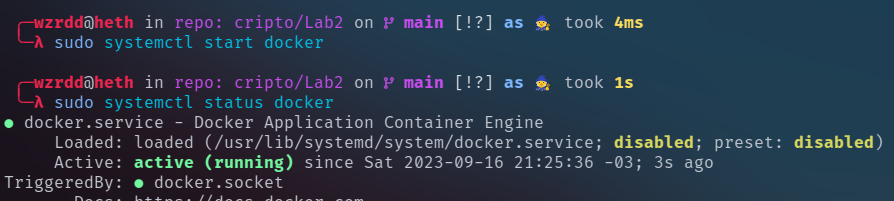
\includegraphics[width=16cm]{images/01-systemctl-docker.png}
  \caption{Iniciación de Docker como servicio}
\end{figure}
En la imagen se ven 2 comandos, el primero como anteriormente se menciona inicia
el servicio de Docker y el segundo muestra el estado actual del servicio, su
estado es ``Active'' e indica que ya está listo para ser usado.

Luego, como indica el \textit{readme} del repositorio de DVWA en Github, para levantar
la aplicación basta con clonar el repositorio en local usando
\begin{listing}
    \BashCode{}
  \begin{lstlisting}
git clone --depth 1 https://github.com/digininja/DVWA
  \end{lstlisting}
\end{listing}
La flag \textit{\-\-depth 1} es opcional y se usa para traer únicamente la rama
principal con una profundidad de 1 commit (véase \code{man git-clone} para más
información). Realizado esto, basta con entrar a la carpeta clonada y ejecutar
\code{docker compose up -d}.
\begin{figure}[H]
  \centering
  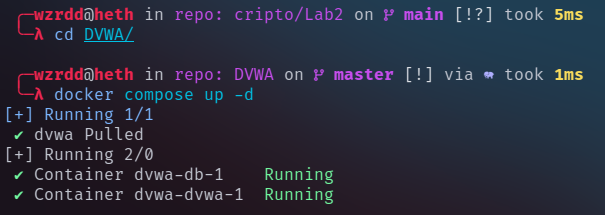
\includegraphics[width=14cm]{images/02-container-running.png}
  \caption{Levantamiento del proyecto como contenedores Docker}
\end{figure}
En la imagen se muestra como, desde el directorio del repositorio clonado se
levantan 2 contenedores: \code{dvwa-db-1} y \code{dvwa-dvwa-1} que corresponden
a la base de datos y a la aplicación respectivamente.

\subsection{Redirección de puertos en docker (dvwa)}
En el archivo compose.yml que describe cómo docker compose va a levantar el
proyecto existen 2 servicios: dvwa (la aplicación a usar) y db (la base da datos
para la persistencia). Únicamente para dvwa se asocia un puerto en el apartado
``ports'' con el valor ``4280:80''. Esto bindea o mapea el puerto 4280 del host
al puerto 80 del contenedor dvwa.
\begin{figure}[H]
  \centering
  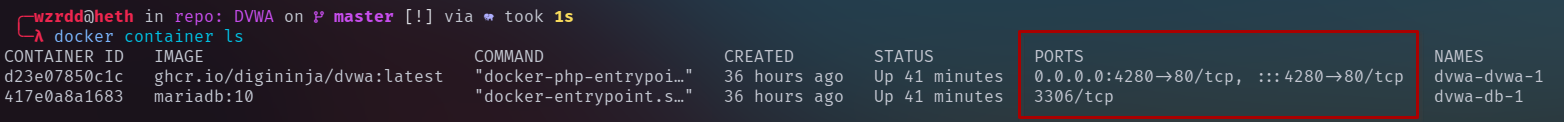
\includegraphics[width=17cm]{images/03-docker-port.png}
  \caption{Listado de los contenedores}
\end{figure}
En la imagen se puede comprobar como se mapea 0.0.0.0 (dirección del host) en su
puerto 4280 (un puerto muy probable que esté desocupado) hacia el puerto 80 del
contenedor (puerto generalmente usado por los proxys HTTP).

\subsection{Obtención de consulta a replicar (burp)}
Para obtener la consulta primero se abre el navegador en la pestaña ``Target''
de BurpSuite lo que inicia un navegador basado en Chromium. Acá accedemos a
localhost:4280 y nos encontramos con un login. En el \textit{readme} del
repositorio de DVWA nos entregan las credenciales admin/password. Ya dentro de
la aplicación entramos a la pestaña ``Brute Force'' o con los mismos resultados
ingresamos a la url http://localhost:4280/vulnerabilities/brute/.

Una vez acá, en BurpSuite se comienza a interceptar desde la pestaña ``Proxy''
\-> ``Intercept''
\begin{figure}[H]
  \centering
  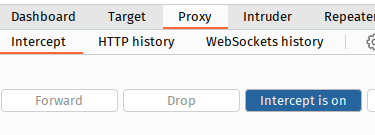
\includegraphics[width=13cm]{images/08-intercept.png}
  \caption{Intercept encendido}
\end{figure}

Con esta configuración volvemos al navegador previamente abierto e intentamos un
login con las credenciales bad/password para forzar un login incorrecto.

\begin{figure}[H]
  \centering
  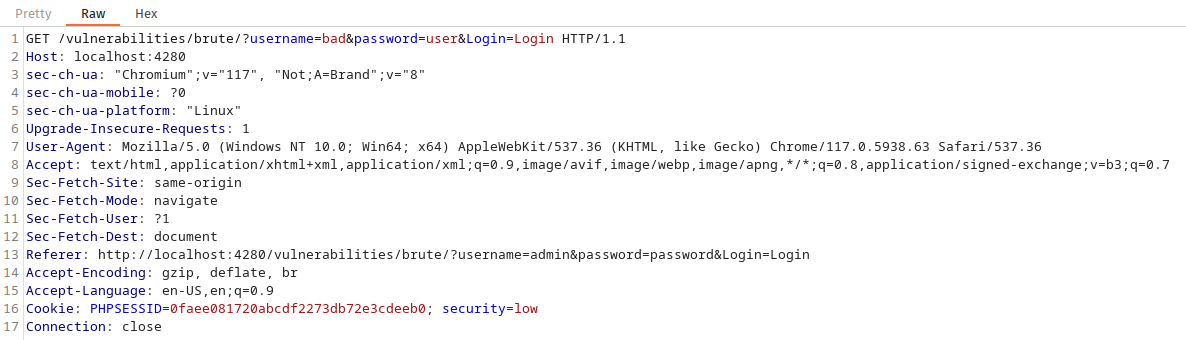
\includegraphics[width=15cm]{images/09-obtencion-consulta.png}
  \caption{Interceptación de la consulta}
\end{figure}

En la imagen se encuentran los headers HTTP con los que se realizó el
\textit{request}. De manera análoga se puede realizar esto mismo en la pestaña
``Proxy'' \-> ``HTTP history'' o en la pestaña ``Target'' si es que las
consultas se realizan en el navegador disponible en esta pestaña. De estas
``HTTP history'' y ``Target'' muestran tanto los headers de los request como el
response.

\subsection{Identificación de campos a modificar (burp)}
Una vez interceptada la consulta, podemos notar que se trata de un request GET
en donde tanto el username como la password son enviados mediante la URL. En
particular, el ejemplo con las credenciales bad/password el request tiene la
forma

\begin{listing}
    \BashCode{}
  \begin{lstlisting}
GET /vulnerabilities/brute/?username=bad&password=user&Login=Login HTTP/1.1
  \end{lstlisting}
\end{listing}

Esta consulta la enviamos a ``Intruder'' con click derecho en la consulta.
Dentro de la pestaña de ``Intruder'' seleccionamos los campos en el request que
irán variando, en este caso username y password. Esto se indica encerrando cada
input con el caracter §.

\begin{figure}[H]
  \centering
  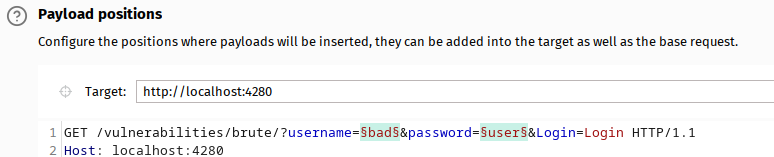
\includegraphics[width=15cm]{images/10-intruder.png}
  \caption{Campos a modificar para el ataque}
\end{figure}

En verde y entre § ambos campos, username y password, serán modificados durante
el ataque.

\subsection{Obtención de diccionarios para el ataque (burp)}
Primero se buscan los posibles nombres de usuarios, probando las mismas
credenciales entregadas en el \textit{readme} del repositorio (que siguen siendo
válidas) podemos obtener un login correcto. En la imagen podemos ver también un
login incorrecto de un usuario y/o una contraseña inválida.
\begin{figure}[H]
  \centering
  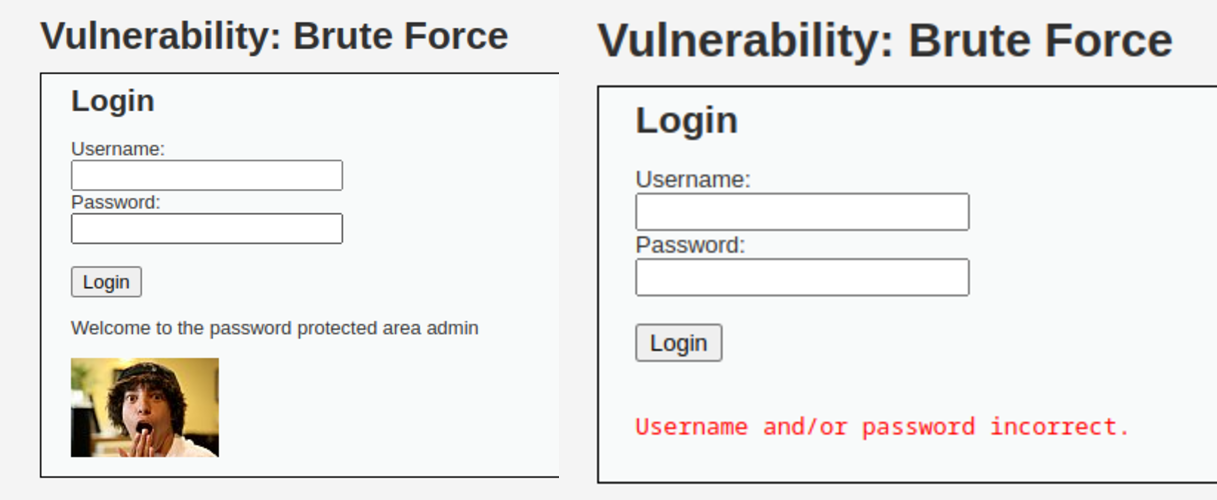
\includegraphics[width=16cm]{images/06-login.png}
  \caption{Login exitoso y fallido respectivamente}
\end{figure}

Revisando la fuente de la imagen de admin podemos notar que pertenece a \\
\code{/hackable/users/admin.jpg}, ruta se puede revisar en el repositorio de
Github del proyecto y entrega 5 nombres de usuarios. Esta será el primer payload
del ataque.

\begin{figure}[H]
  \centering
  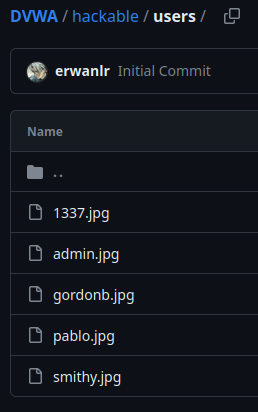
\includegraphics[width=6cm]{images/07-users.png}
  \caption{Nombres de usuarios}
\end{figure}

Para iniciar el ataque por fuerza bruta necesitamos también un diccionario de
contraseñas, usando un diccionario ya construido encontrado en este repositorio
en Github \href{duyet/bruteforce-database}{https://github.com/duyet/bruteforce-database}
se puede usar el que incluye 1.000.000 de contraseñas comunes
(1000000\_password\_seclists.txt). De este archivo se toman los 10.000 primeros
para demorar un tiempo prudente en intentar.

\subsection{Obtención de al menos 2 pares (burp)}
Teniendo ya la lista de usuarios y de contraseñas, se incluyen ambas listas en
la pestaña ``Payloads'' donde el primer conjunto corresponde a los nombres de
usuarios y el segundo conjunto a las contraseñas. Se genera un ataque del tipo
``Cluster Bomb'' que permite 2 o más conjuntos de payloads.

Para comprobar la diferencia entre 1 par válido e inválido se prueba con
admin/password que ya conocemos y admin/bad.

\begin{figure}[H]
  \centering
  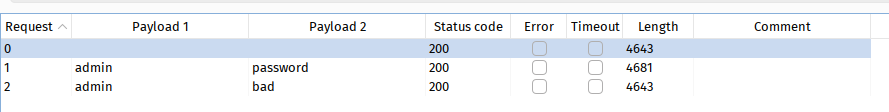
\includegraphics[width=16cm]{images/12-admin-success-and-invalid.png}
  \caption{Primer ataque con par de credenciales válidas e inválidas}
\end{figure}

Estas 2 respuestas son enviadas a la pestaña ``Comparer'', acá se puede ver que
la diferencia es sustancial ya que varían en el mensaje de éxito o error.

\begin{figure}[H]
  \centering
  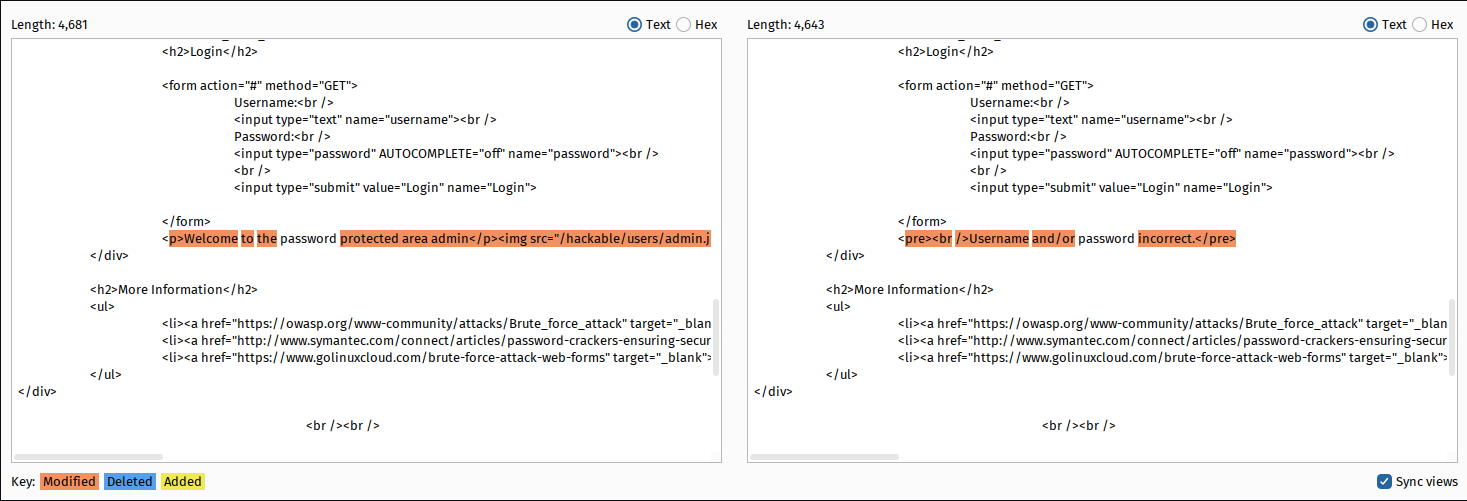
\includegraphics[width=16cm]{images/13-admin-comparer.png}
  \caption{Comparación entre respuesta válida e inválida}
\end{figure}

Con esto se puede comprobar que un mensaje válido tendrá un tamaño de respuesta
mayor porque incluye un mensaje más largo (``\textless p\textgreater Welcome to the password
protected area admin\textless /p\textgreater\textless img src="/hackable/users/admin.jpg" /\textgreater'') e incluye una
imagen. Mientras que un par de credenciales inválidas tiene un mensaje más
conciso (``\textless pre\textgreater \textless br /\textgreater Username and/or password incorrect.\textless /pre\textgreater'').

Un nuevo ataque se genera para los usuarios restantes, en los primeros 60
requests ya se encuentran 3 pares válidos (gordonb/password, smithy/password y
pablo/letmein) y, manualmente se puede detener el ataque para seguir probando
con el último usuario ``1337''.

\begin{figure}[H]
  \centering
  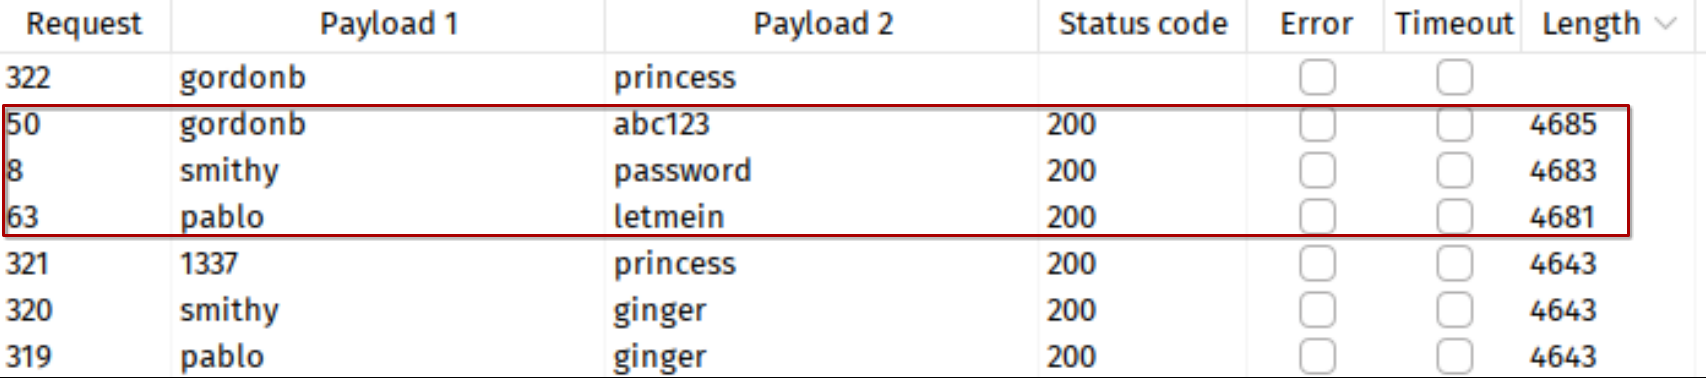
\includegraphics[width=16cm]{images/11-passwords-edited.png}
  \caption{Pares de credenciales válidos}
\end{figure}

Para el último usuario ``1337'' se encuentra la credencial en el código como se
describe en el siguiente párrafo, par de credenciales 1337/charley. En el
diccionario de contraseñas se encuentra en la posición apróximadamente 4000. En
ejecutar 1.000 requests en el computador que se ejecutó fueron 1hr y media
(i5-10310U, 16GB RAM, SSD), es decir, en encontrar la contraseña por fuerza
bruta tomaría 6hrs aproximadamente.

Otra manera de encontrar estas credenciales es, en el repositorio de DVWA en la
carpeta \code{databases/} se encuentran los scripts que crean los usuarios y sus
contraseñas. Tangencial a la experiencia, pero colocar datos sensibles en el
código también es una vulnerabilidad más común de lo que se esperaría.

\begin{figure}[H]
  \centering
  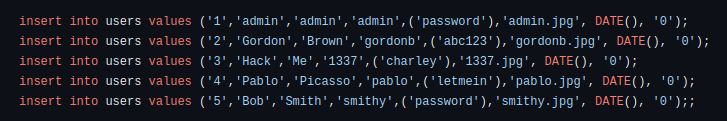
\includegraphics[width=16cm]{images/14-passwords.png}
  \caption{Pares de credenciales válidos desde el código}
\end{figure}

\subsection{Obtención de código de inspect element (curl)}
Se vuelve a la página localhost:4280/vulnerabilities/brute y se repite un
intento de login con las credenciales admin/válidas (password) con las
herramientas de desarrollador abierta y en la pestaña ``Network''.

\begin{figure}[H]
  \centering
  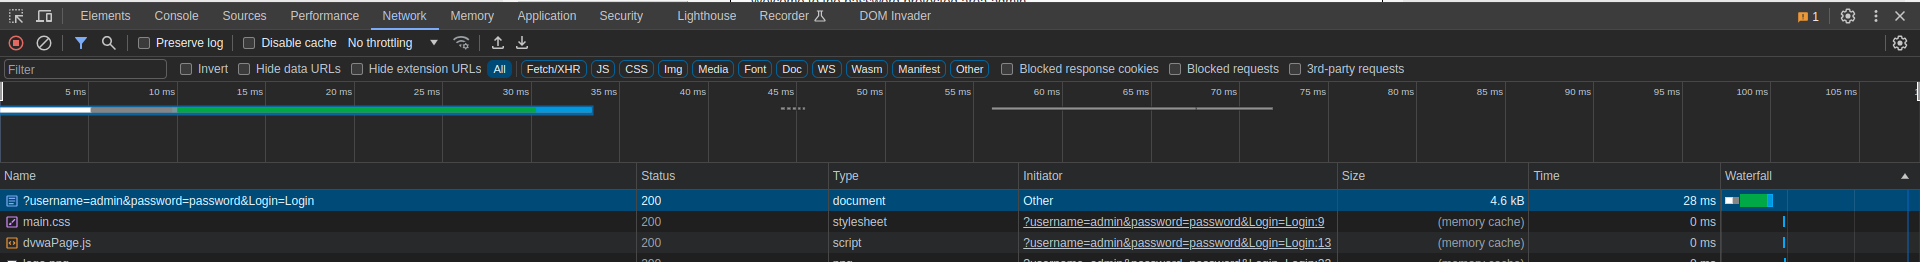
\includegraphics[width=16.5cm]{images/16-curl-inspect.png}
  \caption{Requests de un login visto desde las herramientas de desarrollador}
\end{figure}

Acá se puede ver el request GET del login el cuál se puede copiar directamente a
un comando cURL con click derecho ``Copy'' \-> ``Copy as cURL''. Ejecutamos esto
en terminal redirigiendo el output a un archivo \code{cURL-outputs/output_valido.txt}

\subsection{Utilización de curl por terminal (curl)}
Con el comando copiado se ejecuta desde una terminal.

\begin{figure}[H]
  \centering
  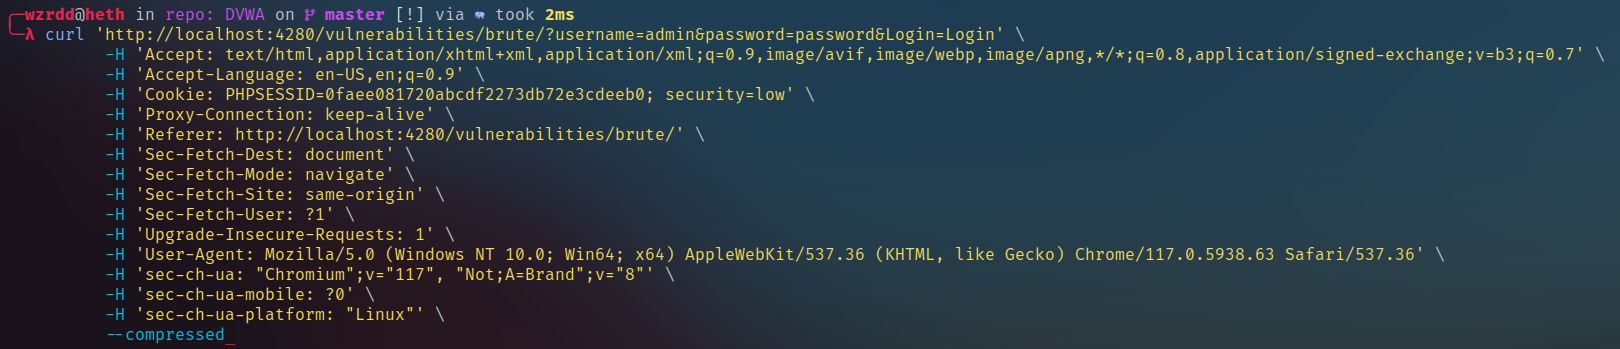
\includegraphics[width=16.5cm]{images/17-curl-command.png}
  \caption{Comando cURL con usuario válido}
\end{figure}

Se repite el comando con un par de credenciales inválidas user/bad y se redirige
al archivo \code{cURL-outputs/output-invalido.txt}. Además, se vuelven a
ejecutar ambos comandos con el flag \code{\-\-head} para obtener los headers de
un request válido e inválido; los resultados son guardados en
\code{cURL-outputs/headers-valid.txt} y \code{cURL-outputs/headers-invalid.txt} respectivamente.

\subsection{Demuestra 5 diferencias (curl)}
Con esto, se usa el comando \code{diff} para buscar diferencia entre ambas
respuestas.

\begin{figure}[H]
  \centering
  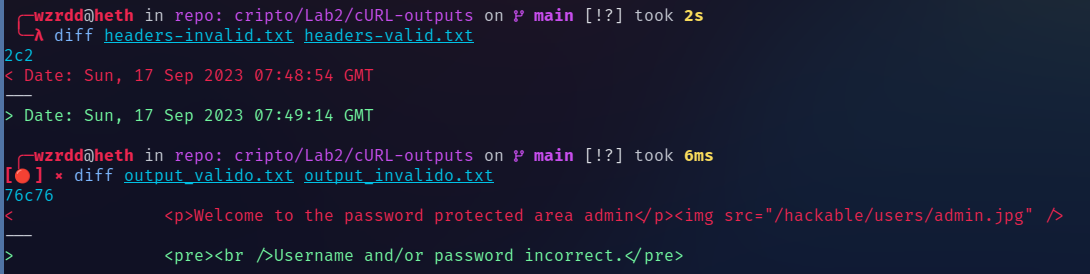
\includegraphics[width=16.5cm]{images/19-diffs-header-and-body.png}
  \caption{Comando diff entre headers y body de las respuestas}
\end{figure}

El comando \code{diff} entrega únicamente las líneas de diferencia entre ambos
archivos,, en rojo el primer archivo que se le entrega y en verde el segundo. En
la imagen se muestra cómo las únicas diferencias entre un request válido y uno
inválido son la hora(porque se realizaron en tiempos distintos) y el mensaje de
éxito o error.

\subsection{Instalación y versión a utilizar (hydra)}
Para instalar Hydra basta con usar \code{sudo pacman -S hydra}.

\begin{figure}[H]
  \centering
  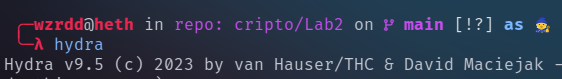
\includegraphics[width=16.5cm]{images/20-hydra-version.png}
  \caption{Versión Hydra}
\end{figure}

Como se nota en la imagen, la versión instalada es la v9.5.

\subsection{Explicación de comando a utilizar (hydra)}
El comando a utilizar sigue de la siguiente forma:

\begin{listing}
    \BashCode{}
  \begin{lstlisting}
hydra -L Diccionarios/users.txt \
-P Diccionarios/passwords-pruned.txt \
127.0.0.1 -s 4280 \
http-get-form "/vulnerabilities/brute/:username=^USER^&password=^PASS^&Login=Login:H=Cookie\: PHPSESSID=c1563ab49faa811139c3bdc9e9580558; security=low:F=Username and/or password incorrect."
  \end{lstlisting}
\end{listing}

Desde lo que se describe:

\begin{itemize}
        \item \code{-L}: Archivo para ser usado como variable \^{}USER\^{}.
        \item \code{-P}: Archivo para ser usado como variable \^{}PASS\^{}.
        \item \code{127.0.0.1 -s 4280}: Host y puerto a utilizar.
        \item \code{http-get-form}: Parámetros del request GET. A saber, la URL
        a consultad, se reutiliza una cookie válida, se pide security=low. El
        parámetro ``F=Username...'' describe una expresión regular a buscar para
        reconocer un request fallido.
\end{itemize}

\subsection{Obtención de al menos 2 pares (hydra)}
Con el comando ya creado y una nueva lista de contraseñas más acotada (168
contraseñas) llamada \code{Diccionarios/passwords-pruned.txt}, se ejecuta:

\begin{figure}[H]
  \centering
  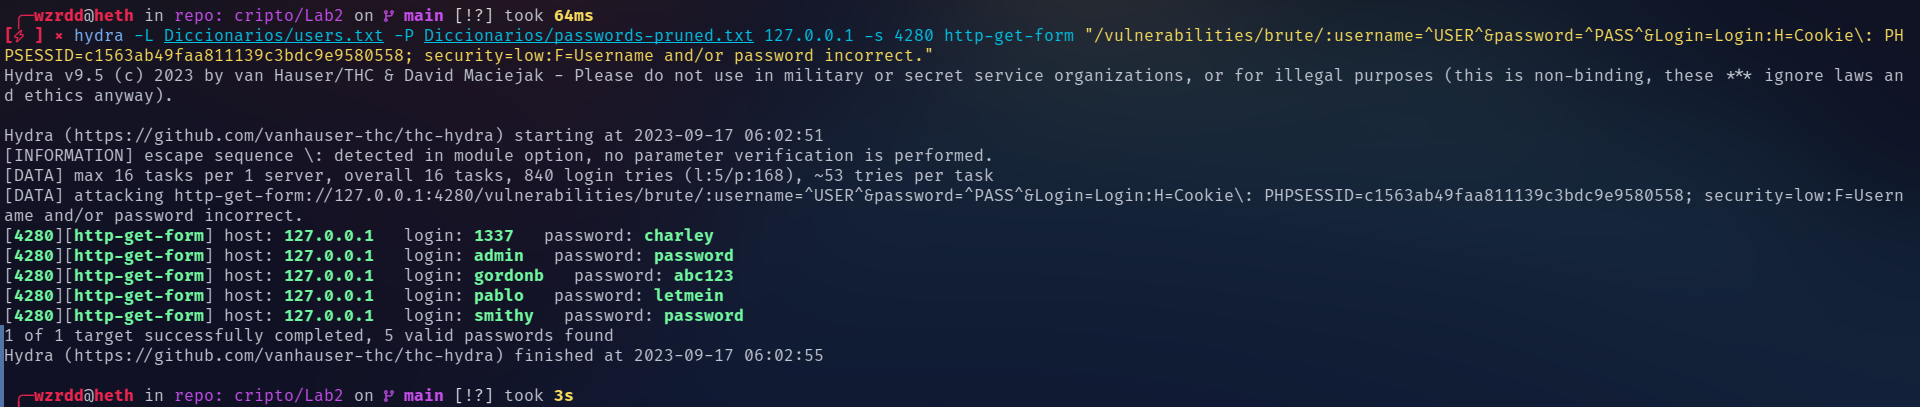
\includegraphics[width=16.5cm]{images/22-hydra-command.png}
  \caption{Ejecución del comando Hydra anteriormente descrito}
\end{figure}

Se agregó en la posición 53 la password para el usuario ``1337'', en la imagen
se puede ver cómo entrega los 5 pares de credenciales válidos.
\subsection{Explicación paquete curl (tráfico)}
Se toma la siguiente serie de paquetes al intentar un login válido.

\begin{figure}[H]
  \centering
  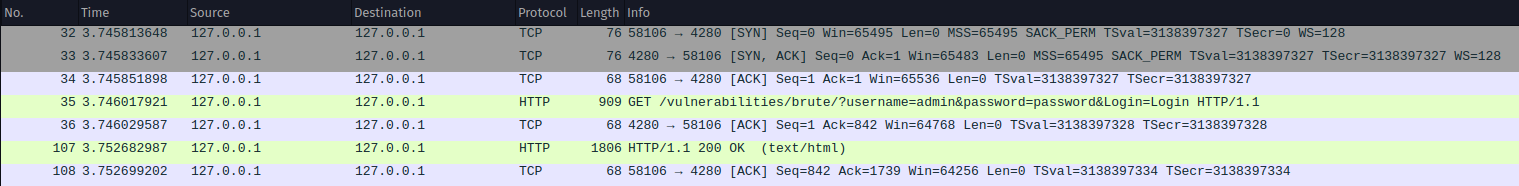
\includegraphics[width=16.5cm]{images/18-curl-packets.png}
  \caption{Estructura de paquetes en un request cURL}
\end{figure}

La estructura inicia con un TCP Handshake de 3 paquetes (SYN, SYN/ACK, ACK
respectivamente) para luego intentar un HTTP request desde el host al
contenedor. El contenedor responde un ACK TCP y retorna un HTTP response. El
ciclo termina con un ACK desde el host al contenedor.

\subsection{Explicación paquete burp (tráfico)}
Se toma la siguiente serie de paquetes al intentar un login válido.

\begin{figure}[H]
  \centering
  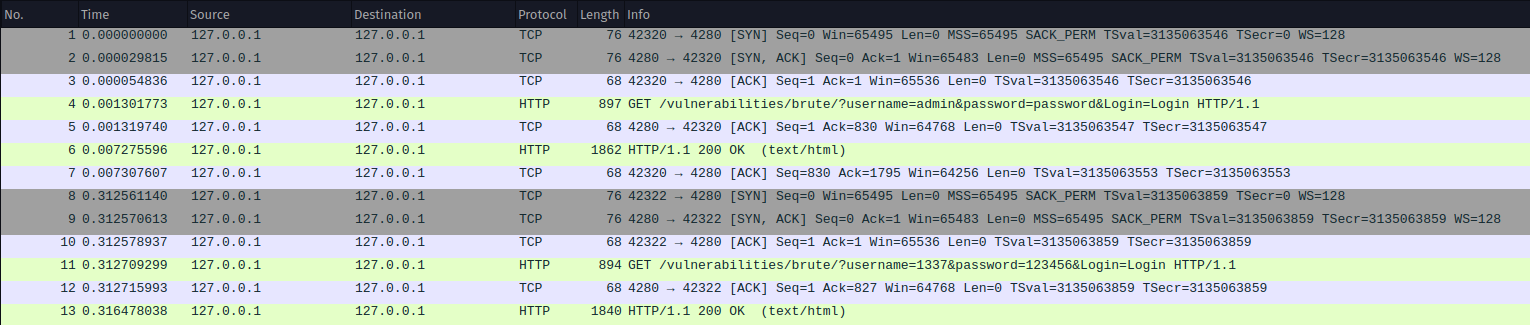
\includegraphics[width=16.5cm]{images/15-burp-packets.png}
  \caption{Estructura de paquetes en un request BurpSuite}
\end{figure}

En la imagen se ven 2 requests inválidos que mantienen la misma estructura que
los request realizados con cURL. Es decir: Un handshake TCP (SYN, SYN/ACK, ACK),
luego un HTTP request desde el Host al contenedor, 1 TCP ACK desde el contenedor
al HOST y un HTTP response, finalmente 1 TCP ACK desde el Host al contenedor.
\subsection{Explicación paquete hydra (tráfico)}
Durante el ataque de fuerza bruta se toma una serie de paquetes de muchos
intentos:

\begin{figure}[H]
  \centering
  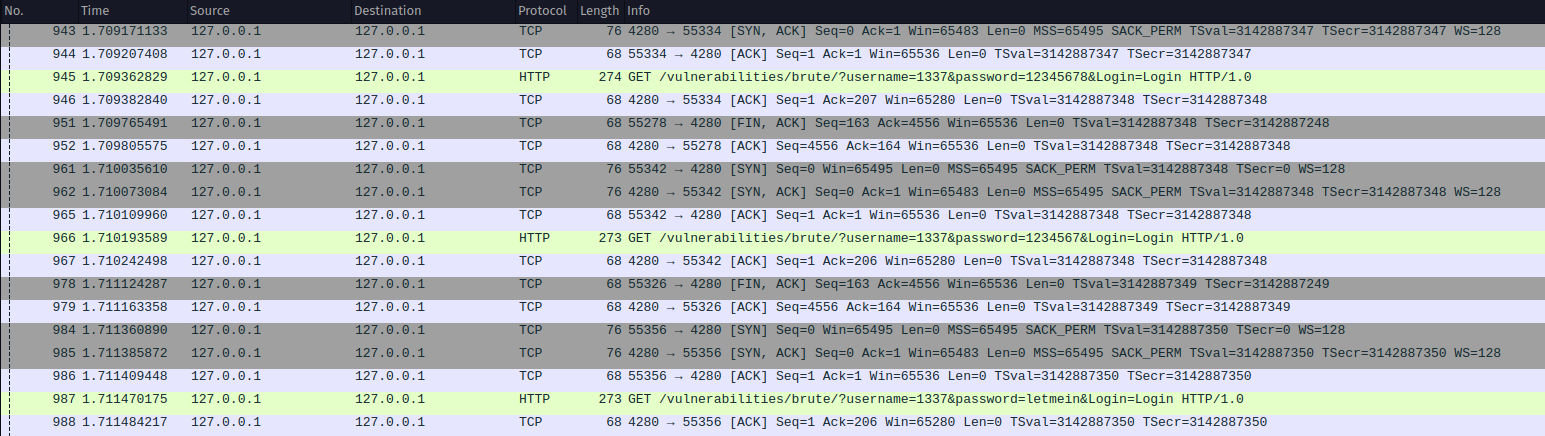
\includegraphics[width=16.5cm]{images/21-hydra-packets.png}
  \caption{Captura de muchos paquetes durante un ataque Brute Force con Hydra}
\end{figure}

En la imagen se puede notar como, aunque siguen un orden similar a cURL y Burp
de paquetes TCP y HTTP. En este caso los requests ocurren de manera concurrente,
lo que dificulta seguir 1 único request.

\subsection{Mención de las diferencias (tráfico)}
La diferencia más notoria en el tráfico entre las 3 aplicaciones es entre Hydra
y cURL/BurpSuite, en la que Hydra genera una mayor cantidad de tráfico más
rápido ya que los requests ocurren de manera concurrente.

En la naturaleza de los paquetes (tamaño), en la secuencia de paquetes TCP y la
respuesta HTTP son prácticamente iguales. Pero en el HTTP request existe una
diferencia notable entre los HTTP requests de Hydra (274 bytes) y de
cUrl/BurpSuite (del orden de los 800 y 900 bytes).

\begin{figure}[H]
  \centering
  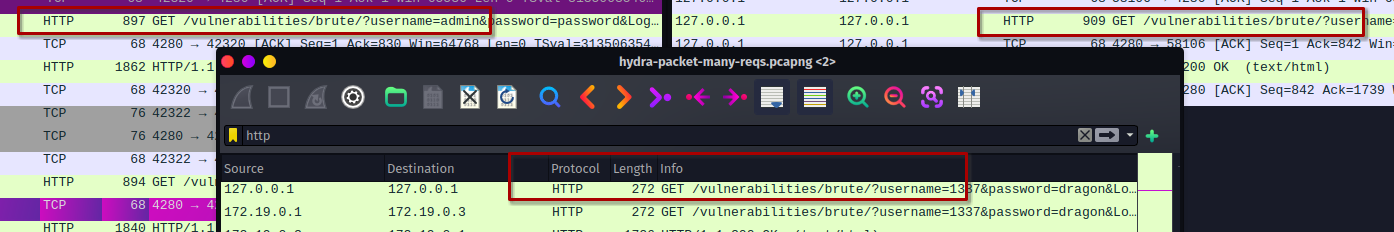
\includegraphics[width=16.5cm]{images/26-diff-in-size.png}
  \caption{Diferencia de tamaño en paquetes HTTP entre Burp (izquierda), cURL
    (derecha) e Hydra (abajo)}
\end{figure}

En el repositorio se encuetran 3 archivos \\
\code{Packets/unsorted-http-packet-<metodo>-as-text.txt} en donde \textless metodo\textgreater puede
ser curl, burp o hydra. En estos 3 archivos se puede ver la diferencia a
inspección simple entre Hydra y los otros 2. En este caso Hydra es bastante más
simple y solo utiliza exáctamente los parámetros del header que se le entrega en
el comando (es decir, la diferencia puede ser mucho menor si se construye de
otra manera el comando para el ataque).

Siguiendo esta línea, para comparar cURL y Burp se toman 2 paquetes HTTP como
texto y además se ordenan. Cabe notar como primera diferencia entre ellos el
orden en que se construyen los parámetros del header.

\begin{figure}[H]
  \centering
  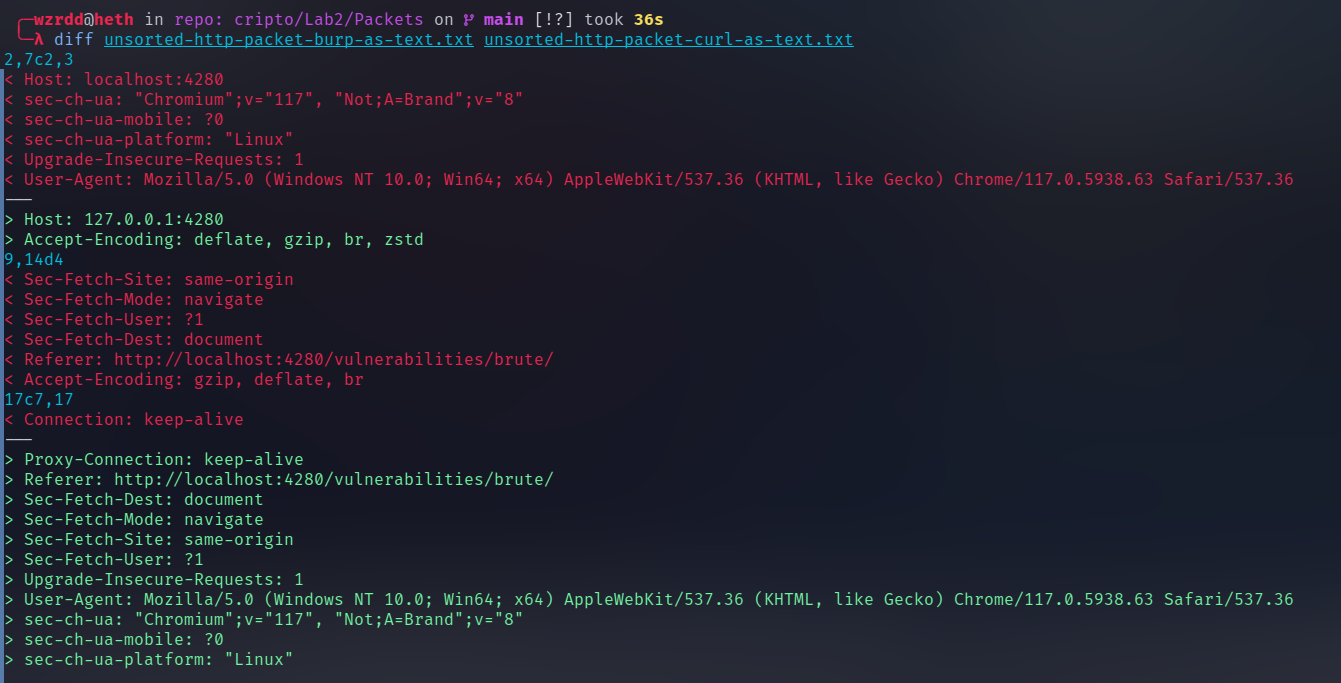
\includegraphics[width=16.5cm]{images/24-unsorted-diff-burp-curl.png}
  \caption{Comando diff entre cURL y Burp desordenado}
\end{figure}

En la imagen se nota como comparten tanto los parámetros del header como sus
valores pero en un orden distinto. Usando \code{sort} en Vim a ambos archivos se
ordena en orden alfabético y se vuelve a ejecutar diff entre ambos.

\begin{figure}[H]
  \centering
  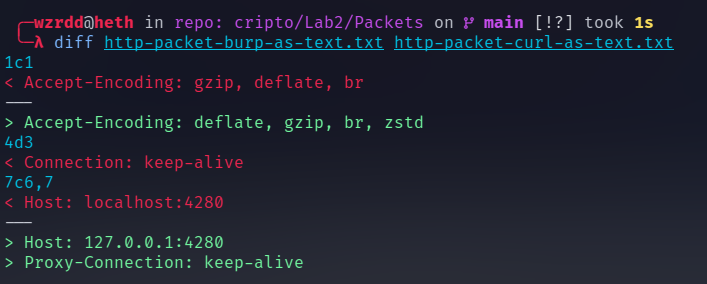
\includegraphics[width=16.5cm]{images/23-diff-burp-curl.png}
  \caption{Comando diff entre cURL y Burp ordenados alfabéticamente}
\end{figure}

Solo 3 diferencias aparecen: el host con el que se construyó son distintos
porque durante la actividad se usó indistintamente localhost y 127.0.0.1. Además
el encoding que aceptan, en su orden y además cURL acepta también \code{zstd} y
además para mantener el keep-alive Burp usa como header ``Connection'' y cURl
usa como header ``Proxy-Connection''

\subsection{Detección de SW (tráfico)}
En esta experiencia sí se puede diferenciar el tráfico entre ambos 3 softwares.
Entre Hydra y los demás por su cadencia en los request, que se solapan mientras
ocurren en paralelo. Y entre cURL y BurpSuite por el orden en el que construyen
los headers para realizar los requests.

Aunque, sí podría realizarse el ejercicio de imitar el request que realiza
BurpSuite usando tanto Hydra como cURL. En el caso de cURL se necesitaría ser
explícito con el encoding aceptados y cambiar el header ``Proxy-Connection'' por
Connection. Aunque el orden de los headers hasta este momento no tiene una forma
de mantenre un orden personalizado, véase
este \href{https://github.com/curl/curl/issues/3282}{Issue en Github} sobre
ordenar los headers, en la discusión también mencionan los TODO del proyecto y,
a la fecha 17 de septiembre del 2023, la capacidad de ordenar los headers
todavía está pendiente.

Para el caso de Hydra, ya que toma verbatim gran parte de los parámetros se
puede asimilar un poco más, tanto copiando los headers en un orden preciso como
en su cantidad. Pero el parámetro ``Host'' Hydra lo coloca al final
del request y Burp al principio. Por lo que sí podría reconocerse por el orden
de los parámetros.

\section*{Conclusiones y comentarios}
A forma de concluir, se puede destacar la diferencia entre los 3 tráficos
generados por BurpSuite, cURL y por Hydra en donde se puede, analizando los
paquetes, obtener mayor información sobre un ataque por fuerza bruta. Al conocer
la herramienta atacante se podría, por ejemplo, crear mejores filtros o tomar
medidas específicas para defender un ataque.

Además, se pudo comprobar durante la experiencia que, aunque un ataque por
fuerza bruta es factible, probar cada combinación de credenciales es lento, de
esto se pueden crear medidas de seguridad como rate-limit para hacer el ataque
aún más lento y además, esconder información como los nombres de usuarios que
inmediatamente multiplican la cantidad de requests a realizar.

Como comentario adicional, se puede extender este trabajo con actividades cómo
intentar imitar el tráfico de BurpSuite con cURL e Hydra, crear diccionarios
especializados para un ataque (enfocado en datos de la empresa, datos
geográficos, demográficos, etc) para darle mayor precisión al ataque, tomar
tiempos de no solo realizar fuerza bruta en la contraseña sino que buscar pares
usuario/contraseña, entre otras actividades.

\section*{Links}
- Repositorio en Github: \href{https://github.com/wzrdd/cripto}{Link}

\end{document}
